%NOTE
\documentclass{article}
\usepackage[margin=1.0in]{geometry}
\usepackage{titling}
\usepackage{graphicx}
\usepackage{float}
\usepackage[T1]{fontenc}

\begin{document}
	
	%%% title
	\setlength{\droptitle}{-5em}
	\title{The Quadrilateral Detective}
	\date{}
	\author{}
	\maketitle
	
	%%% first section
	\section*{Case 2}
	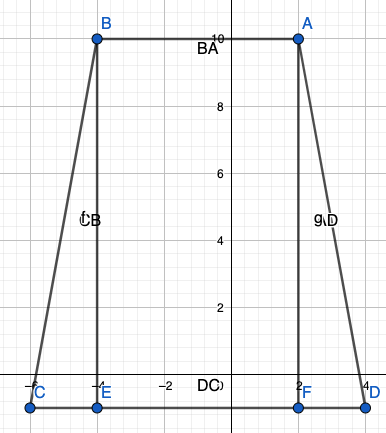
\includegraphics[scale=0.3]{pics/Case2} \newline
	\textbf{Quadrilateral: Isosceles Trapezoid} \newline
	$ABCD$ is a quadrilateral, as it has four sides.\newline
	$AB$ and $CD$ are parallel, as they have the same slope of 0. \newline
	$BC$ and $AD$ have a length of $5\sqrt{5}$ (distance formula) \newline
	$ABCD$ is an \textbf{isosceles trapezoid} as it has $\cong$ bases ($BC$, $AD$) and one pair of parallel sides ($CD$, $AB$). \newline \newline
	\textbf{Area: 88 units$^2$} \newline
	I added auxiliary lines $BE$ and $AF$. \newline
	The area of rectangle $ABEF$ is $6 * 11$, or $66$. \newline
	The area of triangles $CEB$ and $AFD$ are $22$. \newline
	Adding these numbers results in \textbf{88}, which is the area of this trapezoid. 

	\section*{Case 3}
	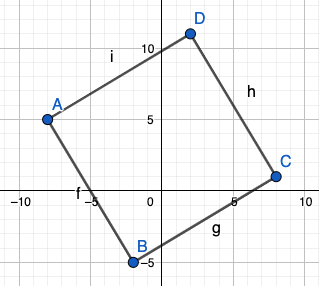
\includegraphics[scale=0.46]{pics/Case3} \newline
	\textbf{Quadrilateral: Square} \newline
	All line segments' lengths are $\sqrt{136}$ (distance formula)\newline
	$AB$ and $CD$ have slopes of $-5/3$ (slope formula) \newline
	$BC$ and $DA$ have slopes of $3/5$ (slope formula) \newline
	All angles are right angles, as perpendicular lines have negative reciprocal slopes. \newline
	$ABCD$ is a square as it has 4 right angles and 4 congruent angles. \newline \newline
	\textbf{Area: 136 units$^2$} \newline
	$\sqrt{136} * \sqrt{136} = $ \textbf{136} 
	
	\section*{Case 4}
	\includegraphics[scale=0.38]{pics/case4} \newline
	\textbf{Quadrilateral: Kite} \newline
	$AB$ and $BC$ are $\sqrt{65}$ in length (distance formula). \newline
	$CD$ and $DA$ are $7\sqrt{13}$ in length (distance formula). \newline
	The slope of line $BD$ is $-1$ (slope formula). \newline
	The slope of line $AC$ is $1$ (slope formula). \newline
	Because these are negative reciprocals of each other, the diagonals ($AC$ and $BD$ are perpendicular). \newline
	As this shape has two sets of $\cong$ sides and perpendicular diagonals, it is a \textbf{kite}. \newline \newline
	\textbf{Area: 154 units$^2$} \newline
	$BD$ has a length of 31.112698, while $AC$ has a length of 9.899495 (distance formula). \newline
	The kite has an area of \textbf{154 units$^2$} (kite area formula).
	
	\section*{Case 5}
	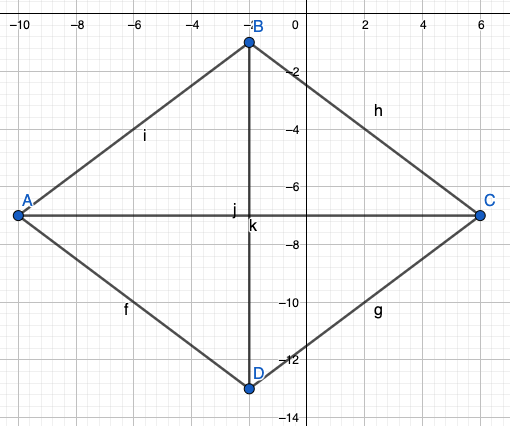
\includegraphics[scale=0.38]{pics/Case5} \newline
	\textbf{Quadrilateral: Rhombus} \newline
	All sides are $\cong$ at 10 units in length. \newline
	$AB$ and $CD$ have a slope of $3/4$, while $BC$ and $DA$ have slopes of $-3/4$. \newline
	This means that $AB$/$CD$ and $BC$/$DA$ are parallel, as they share slopes. \newline
	As this shape has 2 parallel sets of lines and has 4 congruent sides, it is a \textbf{rhombus}. \newline \newline
	\textbf{Area: 96 units$^2$} \newline
	$BD = 12$ and $AC = 16$ (distance formula). \newline
	The rhombus has an area of \textbf{96 units$^2$} (rhombus area formula).
	
	\section*{Case 6}
	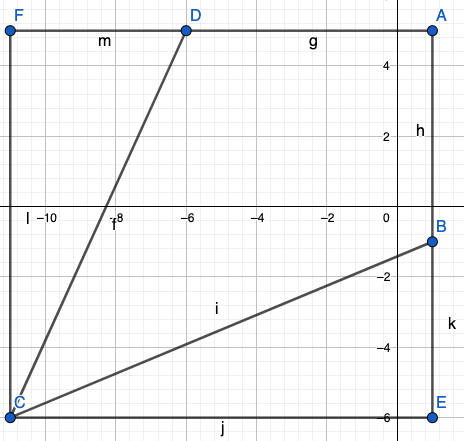
\includegraphics[scale=0.4]{pics/Case6} \newline
	\textbf{Quadrilateral: Parallelogram} \newline
	$AD$, $BC$, $CD$, and $DA$ all have different lengths and slopes. \newline
	This shape does not meet all requirements of any special quadrilaterals, therefore it is a plain \textbf{quadrilateral}. \newline \newline
	\textbf{Area: 74.5 units$^2$} \newline
	Rectangle $FACE$ has an area of 132 (11x12) \newline
	Calculating the area of triangle $FDC$ results in $27.5$, while the area of triangle $CEB$ is $30$. \newline
	Taking away the areas of these triangles to find the true area of the given shape, we get \textbf{74.5} units$^2$.
	\section*{Case 7}
	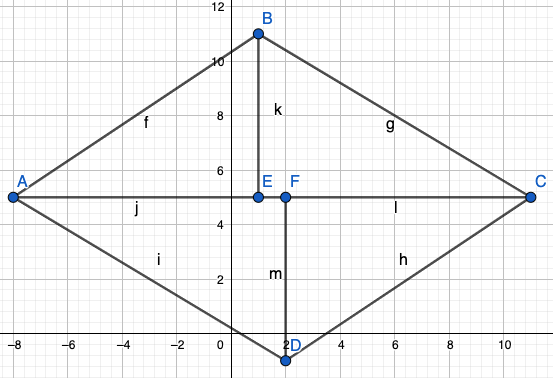
\includegraphics[scale=0.4]{pics/Case7} \newline
	\textbf{Quadrilateral: Parallelogram} \newline
	$AB$ and $DC$ have slopes of $2/3$, while $BC$ and $DA$ have slopes of $-3/5$. \newline
	Because they have the same slopes, $AB$/$DC$ and $BC$/$DA$ are parallel. \newline
	As $ABCD$ has 4 sides and has 2 sets of parallel lines, it is a \textbf{parallelogram}. \newline \newline
	\textbf{Area: 114 units$^2$} \newline
	Triangles $BAE$ and $FCD$ have the area of 27, and triangles $BEC$ and $FAD$ have an area of 30. \newline
	Adding these areas up, the total area of this parallelogram is 114 units$^2$.
	\pagebreak
	\section*{Case 8}
	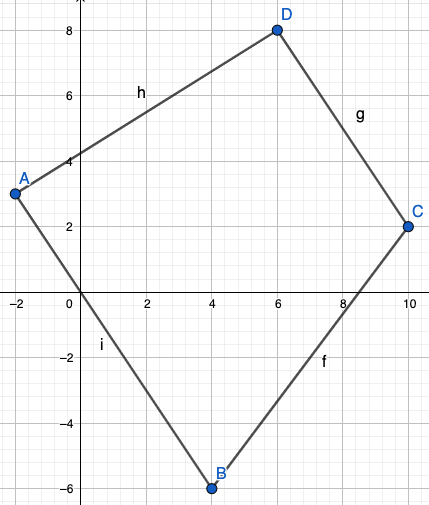
\includegraphics[scale=0.35]{pics/Case8} \newline
	\textbf{Quadrilateral: Trapezoid} \newline
	$DC$ and $AB$ have the same slope of $-3/2$ \newline
	$ABCD$ is a \textbf{trapezoid} because it has 1 set of parallel lines ($DC$ and $AB$) and is a quadrilateral. 
	\section*{Case 9}
	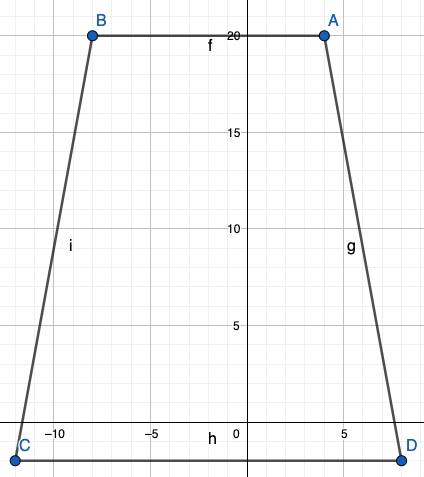
\includegraphics[scale=0.3]{pics/Case9} \newline
	\textbf{Quadrilateral: Isosceles Trapezoid} \newline
	A: (4, 20) B: (-8, 20) C: (-12, -1) D: (8, -2) \newline
	Through the distance formula, the length of $AB$ is 12 units, the lengths of $BC$ and $AD$ are $10\sqrt{5}$, and the length of $CD$ is 20. \newline
	In Case 2's shape, the length of $AB$ was 6 units, the lengths of $BC$ and $AD$ were $5\sqrt{5}$, and the length of $CD$ was 10. \newline
	Here, we can see that these lengths all share the same ratio between Case 2 and 9's shapes: $1:2$. \newline
	This means that dilation would cause these two shapes to perfectly match. \newline
	$AB$ and $CD$ are parallel, as they have the same slope of 0. \newline
	In addition, $ABCD$ is an \textbf{isosceles trapezoid}, just like Case 2, as it has $\cong$ bases ($BC$, $AD$) and one pair of parallel sides ($CD$, $AB$). \newline
	Because all these sides share the same ratios and class of quadrilateral, these shapes are similar.
	\end{document}

